\section{Motivation} % goal?
Albeit the goal stated in the introduction chapter is focused at the method of obtaining quality agents, the motivation for such endavor must be kept in mind. It would be beneficiary for a number of use cases to obtain a system whch, when provided with a sufficient description of an environment and capabilities of agents, could be used to produce ready to be implemented Behavior Trees capable of performing given assignments. Arguably, additional overhead due to implementing the environment \& agents specifications and task description must be taken into account when considering using such system, potentially making the method unfesible in scenarios when the time is of essence. Even then however, one has to weight initial investment into such project against manually designing and adjusting the AI. % is this the right place to mentioned that in some previous research capable trees were found after arguably small number of iterations?

Additionally, there is also one critical advantage to using evolutionary learning methods: the possibility of early termination through end condition. With the right fitness function the option to take an undeveloped tree as a template and improve it becomes perfectly possible. This can be useful in more sophisticated problems, when manual tuning will complement evolutionary method's solution. % to be perfectly honest, i'm not sure if this is the appropriate place to be making such claims - I mean discussing practical advantages.
\section{Formulating a Task}
In order to properly assess feasibility of the system in making, a common task had to be constructed to compare different variations of it against each other. As mentioned before, scenario type chosen for this was a resource gathering.

The premise of this particular scenario was as follows: a number of resource markers (portrayed as flags in the simulation) were scattered across the simulated environment resembling a warehouse. The agents, starting from designated spawn points, are tasked with claiming as many of them as possible against a fixed time limit. \textit{Claiming} in this case was a process consisting of approaching a certain vicinity of a marker, at which point said marker was despawned and marked off as \textit{captured} by an agent initiating the claiming. Making the process instantaneous ensured that markers would be claimed on FCFS (\textit{First-Come, First-Served}) basis.

While the particulars were a subject to fine-tuning numerous times, Figure \ref{fig:x taskoverview} presents the intiial schema of agents' and markers' spawn points.
\begin{figure}[h]
    \centering
    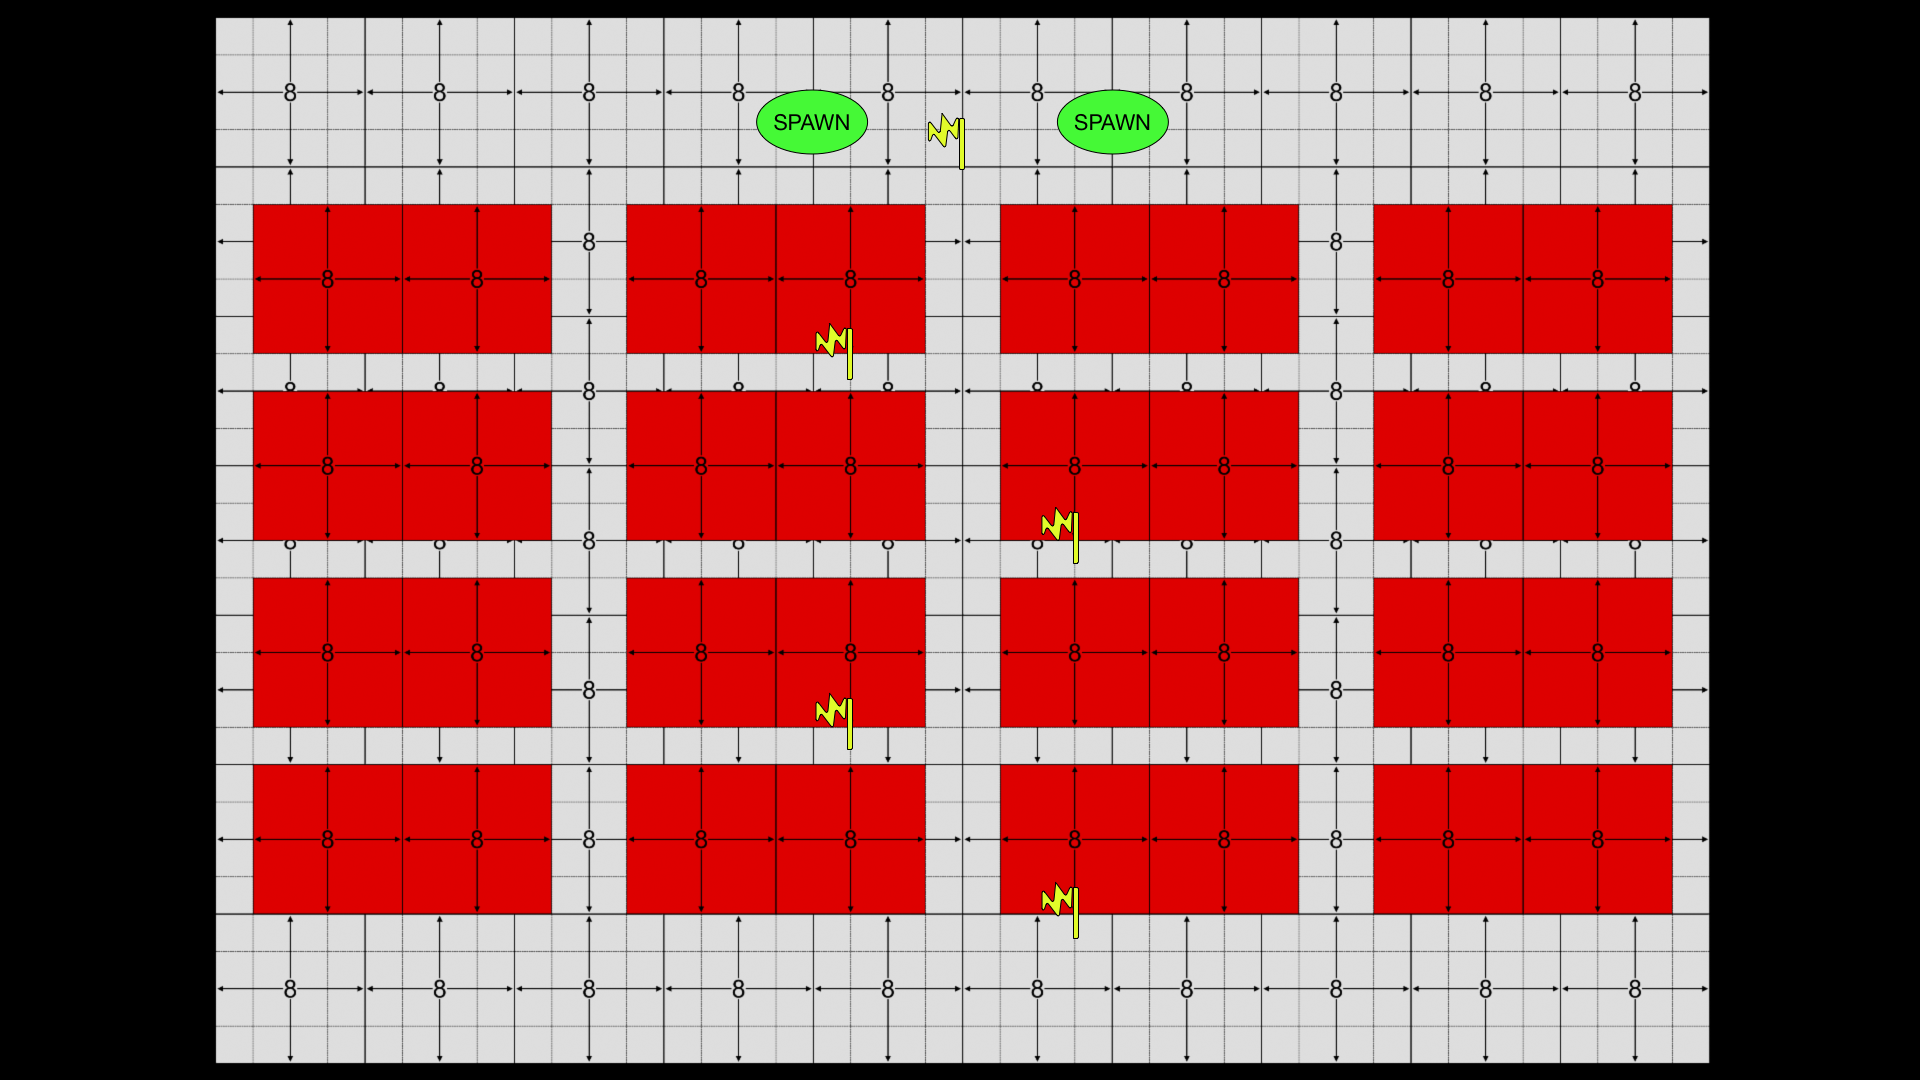
\includegraphics[scale=0.2]{taskoverview}
    \caption{Initial positioning of agents' starting points and resource markers.}
    \label{fig:x taskoverview}
\end{figure}
\section{Introducing Genetic Programming} % change the title
The Genetic Programming module was built on top of FRAIL's existing features, substantially changing the ususal flow of execution to make it suitable for learning processes. Initialisation, evaluation and reproduction steps are all done internally, with evaluation being a step when the actual simulations are run. Since the population was being tested sequentially and the maximum time one could run was 20s (with the possibility to end early, in case all markers were gathered before that time), some testing would take more then 48 hours to complete. A decision was made to increase update frequency of the simulations tenfold, thus guaranteeing simulations would complete afer maximum of 2s.
\subsection{Representation}
In the interest of avoiding integrity requirements and semantic incoherences (which would be undoubtedly caused by genetic operators), a specimen are instances of a specialized class, separated from the actual Behavior Tree implementation. These trees are then parsed during evaluation step to an actual Behavior Tree that is injected to an AI Controller in the simulation.

This simplified implementation allowed for easier manipulation of the trees' components. The nodes are distinguished by their type, but otherwise have all parameters required to operate. While this poses a serious data redundancy, the possibility of freely adding additional node types and ease of operations made this option highly desirable.
\subsection{Genetic Operators} % genetic operations?
\subsubsection{Initialisation}
The population starts as a set of randomly generated specimen of varying size and depth. Each tree generation starts with a random Composite node in root, then the decision is made a at each further step to either add a random Action / Condition node to current root's children or recursively create a random subtree, all bound by a maximum size and maximum depth allowed. This approach provides a varied population while maintaining good balance of Action / Condition and Composite nodes.
\subsubsection{Selection}
The selection method of choice is a regular implementation of Tournament Selection. At each step, a random sample of a given size is selected from the current population and sorted according to a fitness value of the specimen. The first individual from this set is selected for Reproduction purposes.
\subsubsection{Crossover}
On each iteration, two selected specimen have a chance (determined by crossover rate parameter) to produce two children which will be put into the next generation instead of them. The crossover itself is implemented as a exchange of randomly selected nodes (one from each tree) without minding their type nor location.
\subsubsection{Mutation}
Both available mutation methods were implemented: initially, only the possibility for the tree to undergo micromutation is tested - that is implemented by resetting randomly chosen node's parameters to a random values. However, each tree selected for a micromutation process (probability of which is dictated by a mutation rate) has a chance to undergo a macromutation process instead - that, in turn, is determined by a separate, macromutation rate. In this case, micromutation step is replaced entirely with ``Headless Chicken'' mutation.
\subsubsection{Fitness function}
Due to format of the thesis, used fitness function varied in different testing scenarios. Detailed explanations of each will be included in the appropriate sections of Results chapter.
